\documentclass[UTF8,a4paper,12pt]{ctexart}
\usepackage[margin=2.5cm]{geometry}
\usepackage{setspace}
\usepackage{hyperref}
\usepackage{float}
\usepackage{graphicx}
\usepackage{enumitem}
\setstretch{1.35}
\hypersetup{colorlinks=true,linkcolor=black,urlcolor=blue}
\title{关于降低常州制造业企业数字化改造试错成本的建议}
\author{《数字经济概论》期末报告}
\date{}
\begin{document}
\maketitle

常州制造业数字化改造已具备较好基础，但企业仍面临投入回报不确定、人才不足和产业链协同困难。建议把政策支持更多用于小场景验证、岗位实训和上下游数据对接，降低企业试错成本，使财政投入转化为可持续的经营改善。

\section{现状分析}
数字化改造正从设备更新走向业务协同。据国家统计局常州调查队2026年7月发布的资料，2025年常州生产设备数字化率为69.4\%，经营管理数字化率为90.2\%，分别高于全省5.1和1.1个百分点。这说明常州已有较好的应用基础，但两项指标衡量对象不同，不能直接用差值判断改造缺口。\footnote{国家统计局常州调查队：《常州智能制造转型成效明显 仍需协同深化数智融合》，2026年7月10日，\url{https://gdd.changzhou.gov.cn/html/tjjdcd/2026/JECOENJO_0710/7119.html}。}

钟楼区的免费诊断服务是一个典型案例。区工信部门在2025年6月的政府网站访谈中介绍，2024年对55家企业开展诊断，年底累计完成395家工业企业诊断，基本覆盖规上工业企业；并建议企业从一两个痛点场景切入。该案例说明公共服务可以帮助企业明确改造方向，但诊断覆盖率还需与项目落地和经营效果结合评价。\footnote{常州市人民政府网站：《推动钟楼区企业走“智改数转网联”之路》（在线访谈，受访单位为钟楼区人民政府、钟楼区工业和信息化局），2025年6月26日，\url{https://www.changzhou.gov.cn/api/mobile/talk_info.php?theme_id=1865}。}

\section{存在问题}
以下比例均来自常州调查队对112家制造业企业的问卷调研和走访。\footnote{国家统计局常州调查队：《常州智能制造转型成效明显 仍需协同深化数智融合》，2026年7月10日。}

\begin{enumerate}[label=\arabic*、,leftmargin=2em]
\item 投入风险抑制改造意愿。36.6\%的受访企业顾虑系统改造周期长、影响正常生产，33.9\%担心投入与成效不成正比，反映企业需要可验证的收益依据。
\item 人才不足影响系统使用。51.8\%的受访企业将缺乏复合型人才、现有员工操作维护困难列为制约因素，表明采购软件之外，还需补足应用能力。
\item 协同改造难以同步推进。在网络化改造相关问题中，60.7\%的受访企业反映产业链协同难、上下游数字化水平低。单个企业完成改造后，仍可能无法实现跨企业数据联通。
\end{enumerate}

\section{经济机理分析}
第一，固定成本与信息不对称共同提高进入门槛。软件部署、设备接入和流程调整都需要前期支出，小企业较难通过较大业务规模分摊成本。服务商比购买方更了解系统性能，企业难以事先判断适配程度和后续维护费用；投入一旦形成专用系统，又可能成为难以收回的沉没成本。

第二，数字技术与人力资本具有互补性。系统产生数据后，需要员工解释数据并调整排产、维护和管理流程。缺少这些能力，设备与软件投入的边际产出就会下降，仅补贴采购就难以提高实际使用效果。

第三，产业链数字化具有网络效应和协调成本。更多上下游企业接入兼容系统，可以扩大共享信息的价值，但先行企业需要承担接口开发和协商成本，部分收益却由合作方获得，各方都等待对方先投入，可能造成协同不足。

\section{政策建议}
\begin{enumerate}[label=\arabic*、,leftmargin=2em]
\item 由市工信局会同市财政局，在现有“微焕新”项目安排内设置小场景验证支持。\footnote{常州市人民政府办公室：《关于印发〈常州市深化制造业智能化改造数字化转型网络化联接三年行动计划（2025—2027年）〉的通知》，常政办发〔2025〕11号，2025年4月9日成文、4月17日公开，\url{https://www.changzhou.gov.cn/gi_news/592174459911669}。}优先支持质量追溯、设备维护、能耗管理等边界清晰的环节。申请时列明总成本、停机安排和收益指标，分阶段核验实际使用与成效；诊断机构披露与服务商的利益关系，减少借诊断推销设备的情况。
\item 由市人社局、市工信局联合本地职业院校，按照企业岗位需求组织实训。将培训嵌入实施合同，明确服务商交付操作手册、完成现场带教和故障处置演练；以员工能否独立操作、系统是否持续使用评价培训效果。
\item 由市工信局、市数据局组织行业协会和链主企业，先围绕订单、库存、质量追溯等必要内容开展小范围对接。约定接口格式、数据用途、访问权限和退出后的数据导出办法，支持不同服务商接入，降低转换成本。对共性接口和协同验证给予有限支持，按交付周期、库存周转等指标复核效果，企业自行承担日常经营费用，不长期依赖补贴。
\end{enumerate}

\section*{参考文献}
\begin{enumerate}[label={[\arabic*]},leftmargin=2em]
\item 国家统计局常州调查队：《常州智能制造转型成效明显 仍需协同深化数智融合》，2026年7月10日。\url{https://gdd.changzhou.gov.cn/html/tjjdcd/2026/JECOENJO_0710/7119.html}
\item 常州市人民政府网站：《推动钟楼区企业走“智改数转网联”之路》（在线访谈，受访单位为钟楼区人民政府、钟楼区工业和信息化局），2025年6月26日。\url{https://www.changzhou.gov.cn/api/mobile/talk_info.php?theme_id=1865}
\item 常州市人民政府办公室：《关于印发〈常州市深化制造业智能化改造数字化转型网络化联接三年行动计划（2025—2027年）〉的通知》，常政办发〔2025〕11号，2025年4月9日成文、4月17日公开。\url{https://www.changzhou.gov.cn/gi_news/592174459911669}
\end{enumerate}

\section*{AI使用说明}
本文使用ChatGPT进行选题、资料线索检索、结构组织和语言修改，并人工打开政府部门原文核对数据、日期和统计口径。例如，对照参考文献[1]确认，60.7\%是受访企业在网络化改造方面反映产业链协同困难的比例，相关调研涉及112家制造业企业。

\begin{figure}[H]
    \centering
    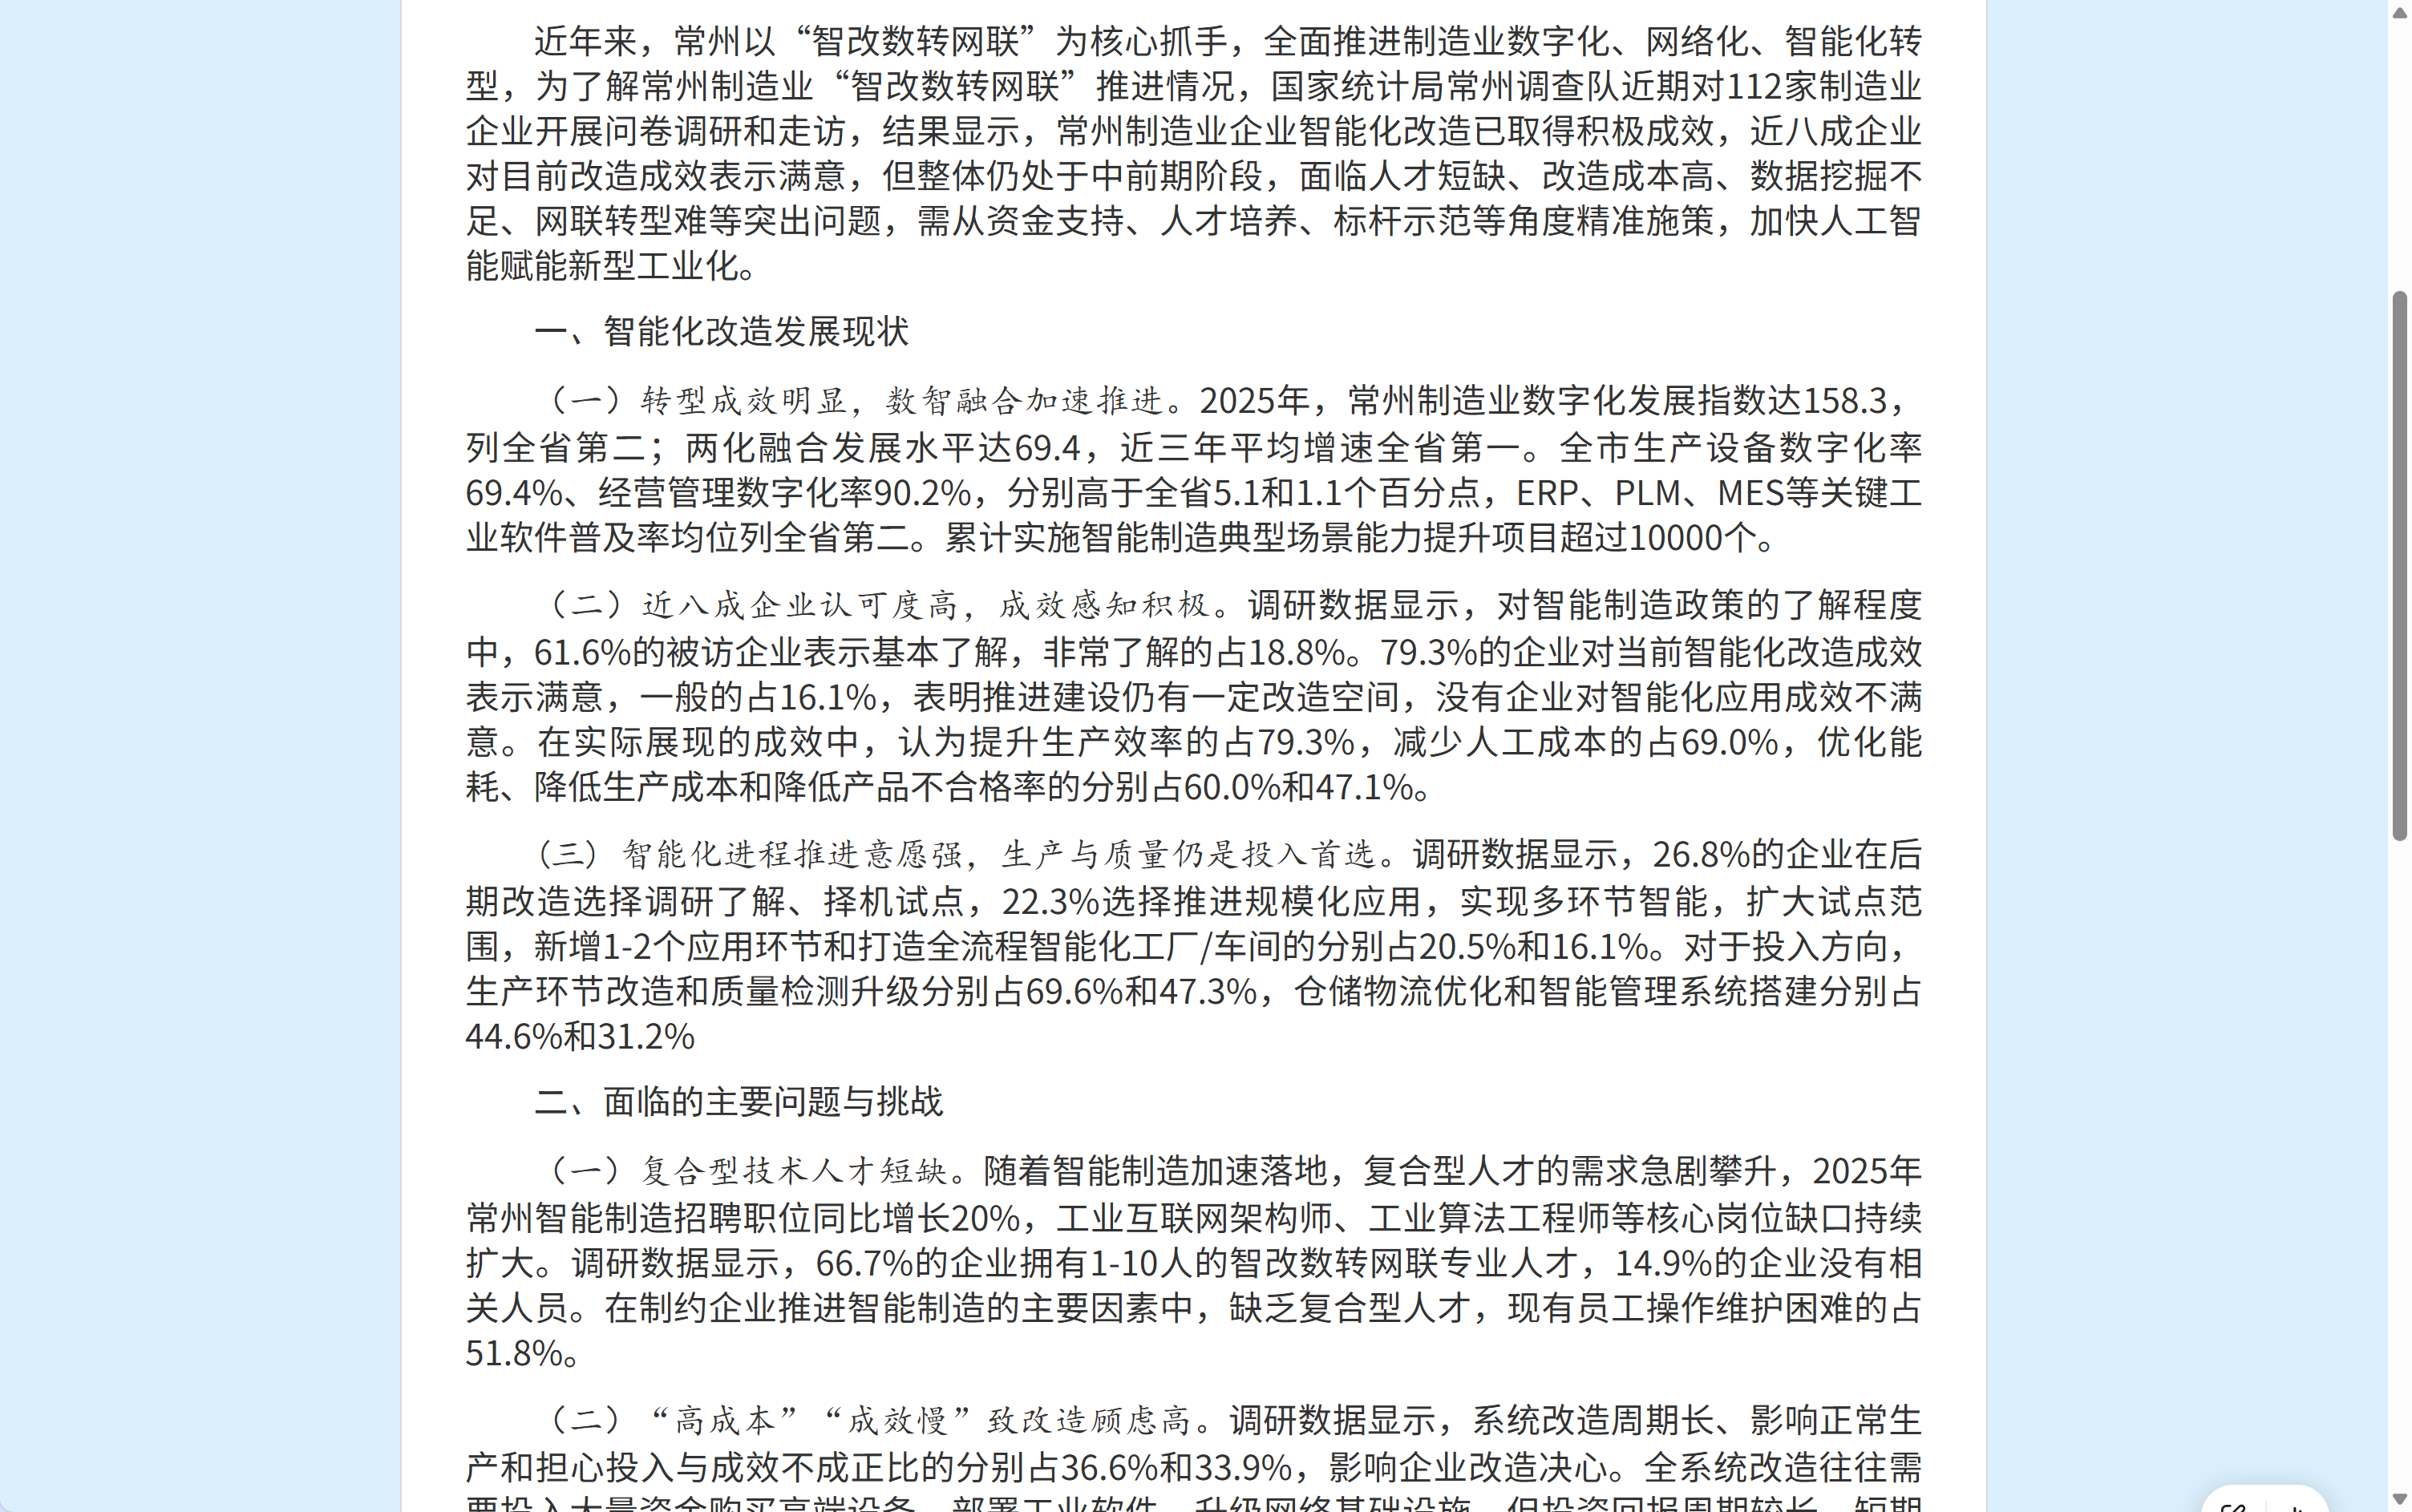
\includegraphics[width=0.8\textwidth]{核实AI提供数据例.png}
    \caption{核实AI提供数据例}
\end{figure}

\end{document}
